%\section{Introducción}

El presente documento describe el desarrollo de un m\'{e}todo para la detecci\'{o}n de anomal\'{i}as en la conducci\'{o}n. Se propone el uso de t\'{e}cnicas de Aprendizaje Autom\'{a}tico para generar un mecanismo que identifique anomal\'{i}as de manejo, de tal modo que \'{e}stas puedan usarse para alertar oportunamente a los conductores y as\'{i} logren correjir sus conductas de manejo.

\vspace{5mm} %5mm vertical space

La idea principal del presente trabajo consiste en aprender el comportamiento normal de conducci\'{o}n, para posteriormente detectar de forma aut\'{o}noma aquellos comportamientos inesperados e informarlos como anomal\'{i}as, de manera que se pueda evitar  un accidente de tr\'{a}nsito o reducir los efectos del mismo.

%Los accidentes de tránsito son resultado del avance tecnológico del mundo moderno, ya que a medida que se han incrementado las distancias entre diferentes puntos, se hizo más necesario el uso del automóvil; lo que llevo a consolidar a éste, como una herramienta esencial para la vida moderna.

\section{Planteamiento del problema}

Debido a las graves secuelas que causan sobre las personas y los altos costos econ\'{o}micos asociados a ellos, los accidentes de tr\'{a}nsito se catalogan como un problema social y de salud p\'{u}blica mundial.

\vspace{5mm} %5mm vertical space

Seg\'{u}n la Organizaci\'{o}n Mundial de Salud (OMS) cada a\~{n}o existen aproximadamente 1,25 millones de muertes a causa de accidentes de tr\'{a}nsito, agregando que la mitad de todas estas victimas son peatones, ciclistas y motociclistas (V\'{e}ase la figura \ref{fig:oms} pag. \pageref{fig:oms}). Asimismo se puede decir que son una de las causas de muerte más importantes en el mundo, y la principal causa de muerte entre personas de edades comprendidas entre los 15 y los 29 años. 

\vspace{5mm} %5mm vertical space

\begin{figure}[h!]
  \begin{center}	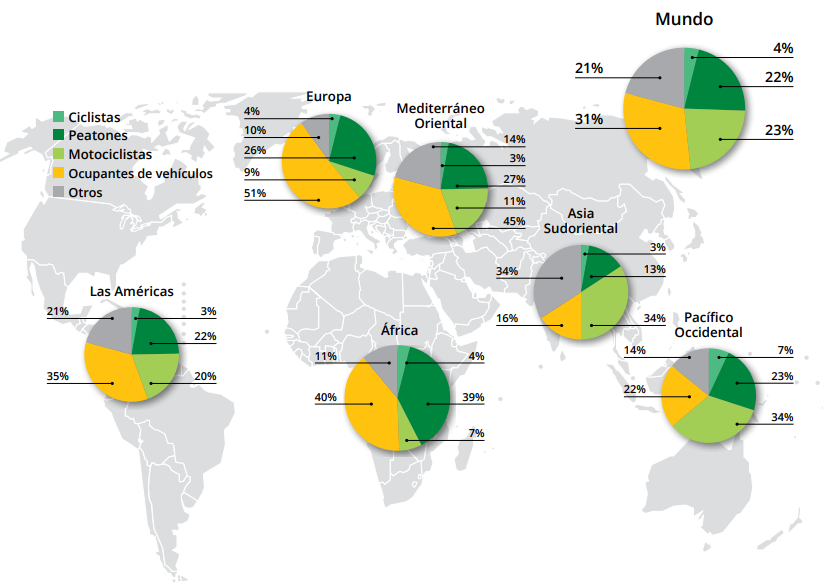
\includegraphics[width=0.9\textwidth]{imagenes/oms1}
  \caption{Muertes por accidentes de tránsito por regi\'{o}n en función del tipo de usuario (2013), OMS}
  \label{fig:oms}  
  \end{center}
\end{figure}

Por otro lado seg\'{u}n la Unidad Operativa de Tr\'{a}nsito de Cochabamba los accidentes registrados en 2017 provocaron la muerte de 200 personas y dejaron aproximadamente 2200 heridos.
	
\vspace{5mm} %5mm vertical space

En la figura \ref{fig:arbol} se muestra las causas por las cuales se ocasiona un accidente de tr\'{a}nsito, se puede observar que gran parte de \'{e}stas se deben al factor humano sin embargo hay otras que conllevan factores medio-ambientales y mec\'{a}nicos, por lo que se hace imposible evitar completamente los mismos. 

\vspace{5mm} %5mm vertical space

Es por ello que se hace necesario el contar con mecanismos para prevenir y/o actuar de forma oportuna ante posibles accidentes de tr\'{a}nsito, motivo por el cual el presente trabajo se centra en estudiar los comportamientos de conducci\'{o}n, para as\'{i} generar alertas al encontrar un comportamiento an\'{o}malo en el manejo, de manera que se pueda evitar o en todo caso minimizar los efectos del mismo.

\begin{figure}[h!]
  \begin{center}	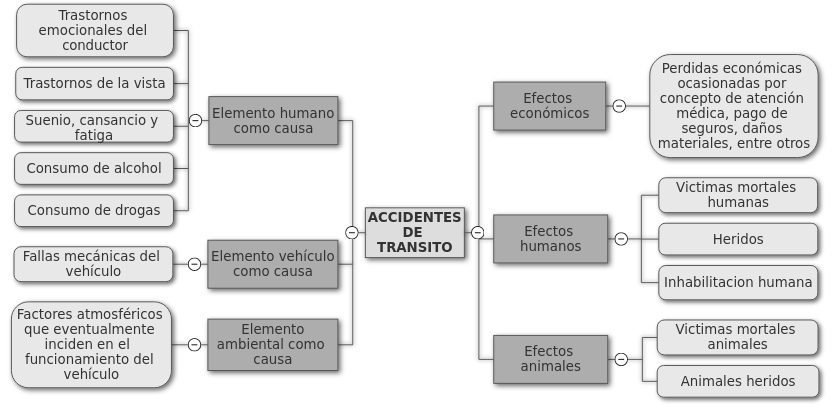
\includegraphics[width=1.0\textwidth]{imagenes/arbol_p}
  \caption{\'{A}rbol de problemas}
  \label{fig:arbol}
  \end{center}
\end{figure}


%El presente trabajo plantea que con la captura de parámetros de manejo de un conductor, mediante el uso de un dispositivo móvil con sistema operativo Android, es posible encontrar patrones de conducción, usando algoritmos de aprendizaje automático,  y determinar si éstos son correctos o en su defecto atentan contra la seguridad de los transeúntes y/o de los otros conductores que comparten las vías con él.

%Por lo tanto se espera que mediante el uso de los sensores de un dispositivo móvil y la aplicación de algoritmos de Aprendizaje Automático sea posible reconocer patrones de conducción, que describan diferentes comportamientos de manejo, y así reconocer automáticamente el incumplimientos de algunas de las normas de circulación y conducción de vehículos en las vías de tránsito con el objetivo de reducir los accidentes viales; ya que si este trabajo se aplicara en la seguridad vial sería de gran ayuda para automatizar la detección de anomalías de conducción y así actuar lo antes posible para evitar un posible accidente.